\documentclass[a4paper,9pt]{article}

% Paquetes básicos
\usepackage[utf8]{inputenc}   % Codificación de caracteres
\usepackage[spanish]{babel}   % Idioma español
\usepackage{graphicx}         % Inclusión de imágenes
\usepackage{amsmath}          % Símbolos matemáticos avanzados
\usepackage{hyperref}         % Hipervínculos
\usepackage{geometry}         % Control de márgenes
\usepackage{cite}             % Citas bibliográficas
\usepackage{setspace}         % Control del interlineado
\usepackage{fancyhdr}         % Encabezados y pies de página
\usepackage{amsmath}
\usepackage{siunitx} % Paquete para usar el símbolo de grados
% Configuración del documento
\geometry{a4paper, margin=1in}
\setlength{\parskip}{1em}
\setlength{\parindent}{0pt}
\onehalfspacing% Interlineado de 1.5

% Configuración del encabezado y pie de página
\pagestyle{fancy}
\fancyhf{}
\fancyhead[L]{Práctica I}
\fancyhead[R]{\thepage}
\fancyfoot[C]{}


%Portada
\begin{document}
\begin{titlepage}
    \centering
    \vspace*{5cm} % Espacio vertical superior
    
    {\large\textbf{Práctica I}}\\[1.5cm] % Título grande
    {\Huge Máquinas Finitas de Estados}\\[1.5cm] % Subtítulo en cursiva
    
    {\Large Marcos Fontenlos\\ % Autores
    Juan Trastoy\\
    Bruno del Campo}\\[2cm] % Espacio después de los autores
    
    {\large \today} % Fecha en letra más pequeña

    \vfill % Espacio flexible para centrar verticalmente

    % Puedes incluir una imagen o logotipo aquí
    % \includegraphics[width=0.3\textwidth]{ruta/de/la/imagen.jpg}
    
\end{titlepage}
\newpage
\tableofcontents
\newpage

% 1. Introducción
\section{Introducción}
El objetivo de la práctica es diseñar un comportamiento reactivo de un robot por medio de una máquina finita de estados de forma que nuestro robot sea capaz de resolver por sí mismo un laberinto estándar de una complejidad no muy alta. Pondremos en práctica distintos algoritmos para ajustar el comportamiento del robot de forma que realice acciones de forma inteligente. 

\paragraph{}

Para construir un comportamiento correcto y optimizado para que nuestro robot de ejemplo consiga salir de cualquier laberinto podremos utilizar diversas técnicas y algoritmos de búsqueda. El más sencillo en cuanto a complejidad y el primero que hemos estudiado ha sido el seguidor de paredes, pero no ha sido al que hemos recurrido finalmente. Gracias a este algoritmo podemos resolver cualquier laberinto de forma sencilla únicamente siguiendo un proceso de búsqueda y seguimiento de una pared concreta, siempre y cuando ese laberinto este completamente conectado, a saber, que todos sus caminos estén conectados y no contenga islas aisladas. El problema de esta solución es que pese a que tendrá una tasa de éxito absoluta independientemente de la complejidad del laberinto, el robot tardará mucho en llegar a la meta, y es probable que pase varias veces por el mismo sitio, lo cual es un comportamiento indeseado; es decir, el algoritmo \textit{follower} de paredes es muy robusto pero poco eficiente, y solo se puede aplicar a laberintos unicursales o perfectos.
\paragraph{}
Indagando un poco más en algoritmos que pudiésemos utilizar decidimos hacer una implementación lógica del algoritmo de Trémaux (no implementandolo al final). Este algoritmo es una opción muy interesante para resolver laberintos, pues es capaz de resolver cualquier laberinto, sea unicursal o multicursal o aun que contenga bucles, en un tiempo razonable. Esto sucede gracias a que el algoritmo de Tremaux emplea el uso de memoria para recordar los caminos que ha recorrido y los que no, de forma que no se repita en ningún momento. La complejidad de este algoritmo es mayor que la del seguidor de paredes, pero es mucho más eficiente y rápido. Sin embargo, la ventaja de este algoritmo es también su mayor desventaja, pues la memoria que emplea es un recurso limitado y si el laberinto es muy grande o complejo el robot podría quedarse sin memoria y no ser capaz de resolver el laberinto; además requiere de un cálculo más complejo basado en la odometría que se obtiene en base a las mediciones de los sensores y a la respuesta esperada de la acción de movimiento. Es por eso que en según que laberintos es mejor aplicar un algoritmo puramente reactivo como el seguidor de paredes, o bien un algoritmo más complejo: dependerá de las necesidades del problema.
\paragraph{}
Por último, desarrollamos un comportamiento reactivo únicamente con la distancia. Nos dimos cuenta de que únicamente la información del láser del robot podía ser suficiente para darle a nuestro robot un comportamiento lo suficientemente inteligente como para salir del laberinto empleando únicamente muestras de rangos independientes. Este planteamiento no es, a priori, capaz de resolver laberintos, pues no tiene en cuanta la topología del laberinto, ni garantiza la marcha adente (existe el riesgo de que el robot vuelva hacia atrás ante estructuras como callejones sin salida), pero es un buen punto de partida para desarrollar un algoritmo más complejo que pueda resolver laberintos de forma eficiente y rápida. 

% 2. Planteamiento y desarrollo
\section{Planteamiento, modelización y desarrollo}
\subsection{Planteamiento}
Los pasos a seguir para resolver la práctica fueron, en primer lugar, escoger el algoritmo con el que moveremos al robot, pues de este dependerá en gran medida el comportamiento que le debamos de dar al robot posteriormente y el diseño de la máquina de estados que debemos construír; en ningún caso podremos diseñar una máquina de estados precisa si no tenemos claro las acciones que podrá realizar nuestro robot pues diferentes metodologías implican diferentes posibilidades para el robot.

\subsection{Máquina de estados}
A lo largo de esta práctica hemos experimentado con diferentes máquinas de estados en busca de una que sea lo más polivalente posible pero siempre conservando cierta simplicidad considerando la dimensión del tiempo de desarrollo e implementación. En nuestra primera máquina de estados contábamos con implementar un seguidor simple de paredes, lo que nos hizo cambiar de parecer fué la cantidad de posibilidades que debíamos 
considerar en los aspectos de movimiento, distancias... para que el robot fuese capaz de resolver todo tipo de 
laberintos comenzando desde cualquier posición. Por ello decidimos buscar otras posibilidades que fuesen más 
potentes y que exprimiesen al máximo las capacidades de nuestro robot.  

\subsubsection{Seguidor de paredes}
Fueron varias las ideas que tuvimos para empezar a construír la máquina de estados que definiese un seguidor 
de paredes, al inicio de la práctica teníamos la idea de crear una máquina de estados secuencial para que 
la conversión a programa fuese casi automática pero posteriormente decidimos que si hacíamos una máquina 
con diferentes estados que a su vez tuviesen otros estados dentro de ellos mismos podríamos simplificar las 
cosas a la hora de diseñarla. Por tanto, nuestro primer esquema de máquina tiene 3 estados principales, de los 
cuales se derivan otros que dan un escalón de profundidad al comportamiento empleando una herencia.
[Figura~\ref{fig:seguidor1}]

\begin{figure}[h!]
    \centering
    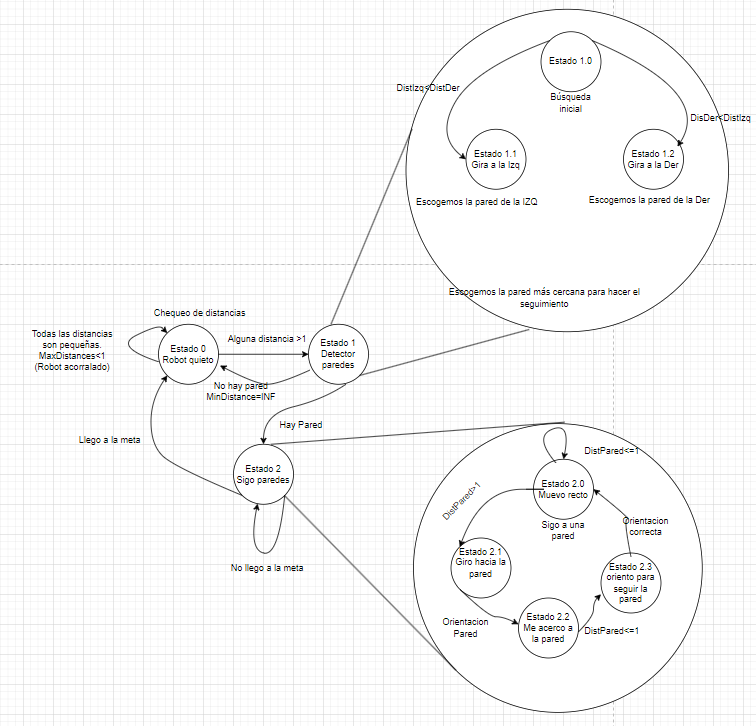
\includegraphics[width=0.8\textwidth]{Imágenes Memoria/Diagrama_Sigue_Paredes_prueba.PNG}
    \caption{Primer boceto de nuestra máquina de estados sigue paredes}
    \label{fig:seguidor1}
\end{figure}

\paragraph{}

En base a este planteamiento inicial fuimos puliendo la máquina para que considerase multitud de posibilidades para resolver el laberinto para al final conseguir lo siguiente:

\begin{figure}[h!]
    \centering
    \begin{minipage}{0.45\textwidth}
        \centering
        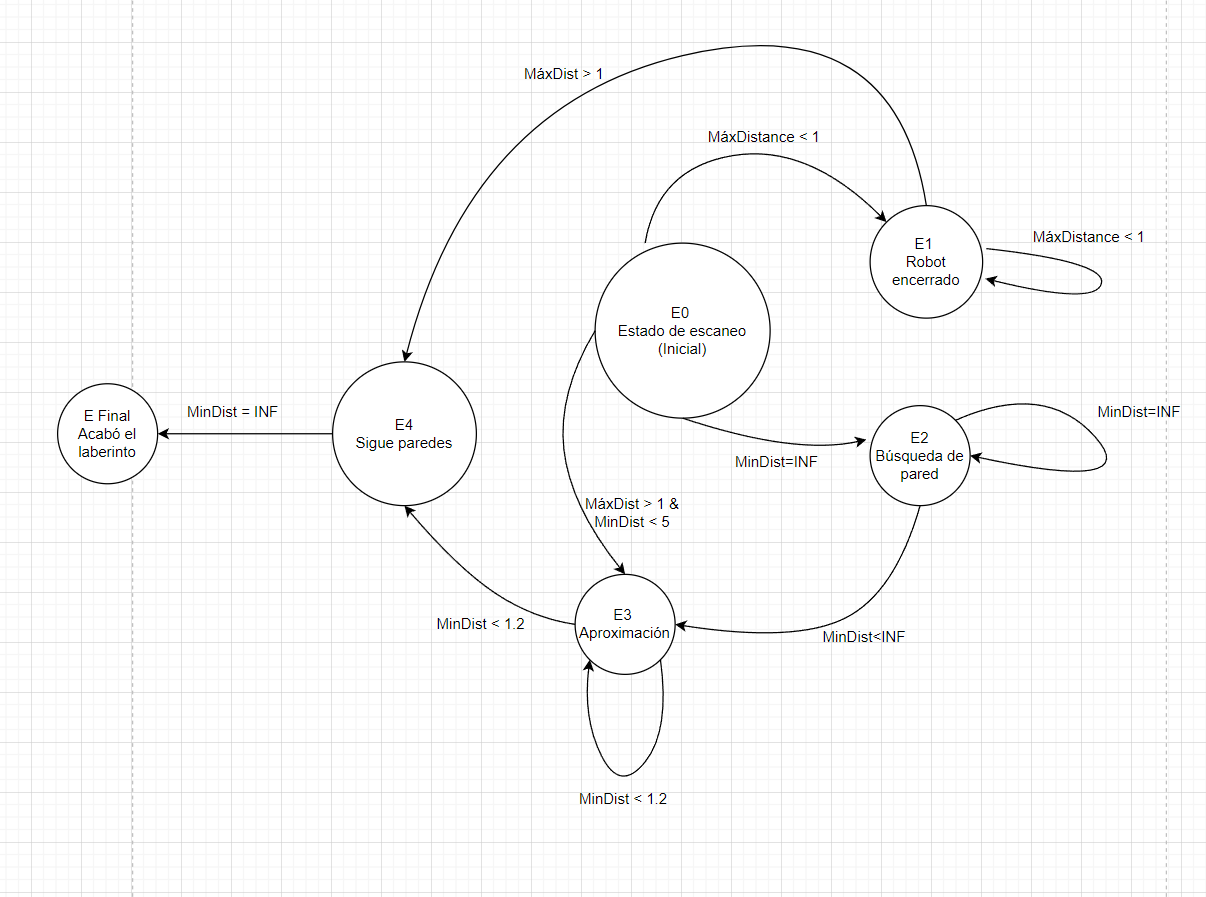
\includegraphics[width=\textwidth]{Imágenes Memoria/Diagrama_Sigue_Paredes_2.PNG}
        \caption{Máquina de estados final del sigue paredes}
        \label{fig:Maquina de estados sigue-paredes}
    \end{minipage}%
    \hspace{0.05\textwidth} % Espacio entre las dos imágenes
    \begin{minipage}{0.45\textwidth}
        \centering
        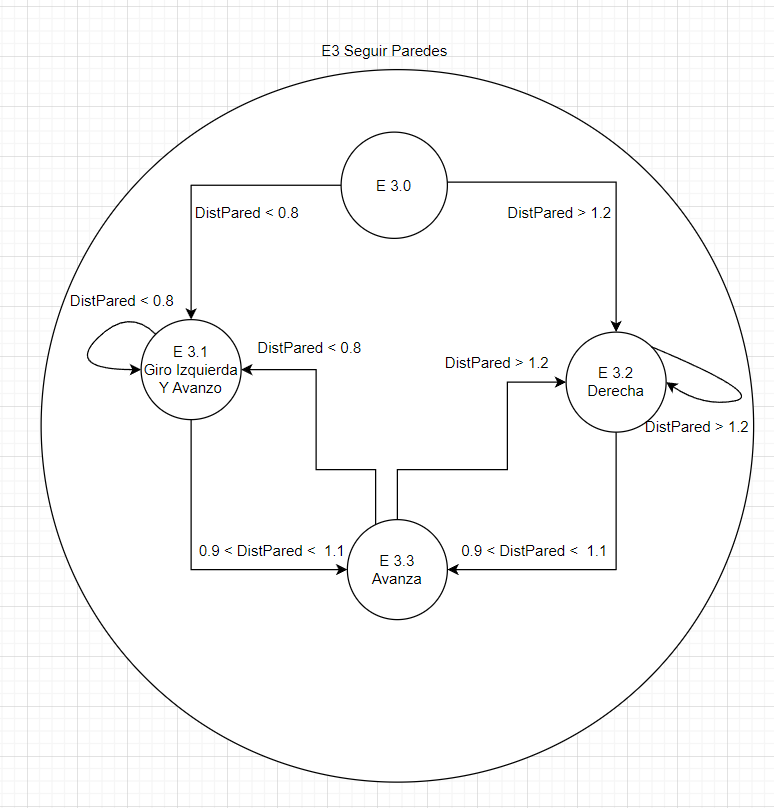
\includegraphics[width=\textwidth]{Imágenes Memoria/Estado_Sigue_Paredes_2.PNG}
        \caption{Subestado}
        \label{fig:Subestado}
    \end{minipage}
\end{figure}

El estado inicial será de reposo del robot, en este estado el robot no se mueve pero sí que es consciente de las distancias de los objetos a su alrededor. Pudiera parecer que es un estado innecesario dado el tipo de problema que queremos afrontar pero no debemos olvidar que no sabemos en que tipo de laberinto puede encontrarse nuestro robot, sería ineficiente que el robot se moviese si se encuentra en un espacio cerrado o frente a una salida cerrada nada más entrar al laberinto, por tanto es una buena implementación que lo primero que haga el robot nada más empiece a funcionar sea evaluar las distancias para saber en qué situación se encuentra.
\paragraph{}
Dependiendo del resultado de la evaluación del primer estado, podremos decidir el comportamiento más sensato. Como el robot solo evalúa la distancia en un rango de \SI{180}{\degree}, nos falta información completa del entorno. Por suerte, podemos solucionar este problema girando el robot; de esta forma, si giramos \SI{180}{\degree} el robot, tendremos un escaneo de \SI{360}{\degree} completo. 

Este escaneo total solo será necesario en caso de que todas las distancias que recibimos en una primera instancia sean infinitas (no hay paredes ni objetos enfrente) o sean menores que un rango (el robot se encuentra entre paredes). En el primer caso, el robot debería moverse hacia delante en busca de paredes de forma indefinida hasta que encuentre una pared. En el segundo caso, el robot debe girar hasta que en un rango que hemos estimado de unos \SI{60}{\degree} enfrente del robot tenga una distancia mínima mayor a un rango que estimemos. De esta forma, podemos controlar el giro con mayor precisión.

\paragraph{}

Una vez hayamos superado estas situaciones significará que ya estamos dentro del laberinto y comenzaremos la tarea de aproximarnos a una pared, que es a su vez un nuevo estado, para ello, nos orientaremos hacia la dirección de mínima distancia y nos aproximaremos hasta llegar a una distancia prudencial de la misma, pero suficiente para ser capaces de seguir la pared con precisión. En el momento en el que estemos a esa distancia pasaremos al siguiente estado; el seguidor de paredes.
\paragraph{}
Podemos considerar este estado el más importante de todos ya que en su concepción decidimos que contuviese en su interior toda a lógica de movimiento del robot. Las directrices: derecha, izquierda y delante son parte de este estado, que evaluará la distancia a la pared de forma que el robot se mantenga siempre en un intervalo de distancia con la pared. En este momento el robot solo debe aplicar las directrices de forma lógica para ser capaz de llegar a la salida del laberinto.
\paragraph{}
Para saber que el robot está efectivamente en el final del laberinto, definiremos un nuevo estado al cual sólo llegaremos si todas las distancias detectadas por el lidar son infinitas, pues esta es la información que obtendremos si el robot ha llegado a la salida.

Como podemos observar, hay bastantes estados posibles para este algoritmo de búsqueda, lo cual, puede complicarnos la parte de programación del mismo, además, imprecisiones en las medidas del robot podrían llevarnos a un comportamiento indeseado por lo que este algoritmo, pese a ser eficaz es poco eficiente y poco robusto. 

\subsubsection{Algoritmo de Trémaux}
El algoritmo de Trémaux es específico para la resolución de problemas del tipo laberinto. Este algoritmo nos permite definir una máquina de estados regida por unas máximas y que, siempre que no rompamos estas máximas, funcionará para resolver el algoritmo. Básicamente el algoritmo de Trémaux es una forma particular de la búsqueda en profundidad sobre un grafo, en este caso, el laberinto. Se diferencia de la DFS en que no necesariamente explora todos los nodos del grafo, sino que se centra en encontrar una salida; además tambien se diferencian en que el algoritmo de Trémaux no solo retrocede cuando llega a un callejón sin salida, sino que también lo hace cuando detecta qu un camino ya ha sido explorado desde la intersección a la que llega.
\paragraph{}
Las reglas del algoritmo de Trémaux son las siguientes:
\begin{enumerate}
    \item No se puede pasar dos veces por el mismo camino:=(negro).
    \item Si llega a un nodo desconocido (no visitado), tomar cualquier camino.
    \item Si llega a una intersección (nodo) que ya hemos visitado desde un camino no recorrido (blanco), o si se alcanza un callejón sin salida debemos retroceder.
    \item Si, en cambio, llega a una intersección que ya hemos visitado desde un camino recorrido (gris), se debe tomar un camino no visitado (blanco) o, si no existe, tomar cualquier camino (gris, si no existe, negro).
\end{enumerate}
La implementación de este algoritmo en una maquina de estados finitos tiene que conjugarse con los estados que controlan el movimiento del robot y las diferentes situaciones con las que se puede encontrar. Si bien este algoritmo garantiza la resolución del laberinto, es necesario contemplar estados y subestados dedicados al movimiento puro y otros que conjuguen ese control con el cumplimiento de los requerimientos del algoritmo. En una primera aproximación lógica se ha dibujado una FMS con los estados Inicio, Exploración, Análisis, Retroceso, Finalizado y Excepción.
\paragraph{}
Todos los condicionales de la máquina en su nivel más abstracto (el que se corresponde con la lógica del algoritmo) se fundamentan en una clase Nodo. Cada intersección se considera como un nodo que posee los atributos de posición (por odometría) y de estado de los caminos (blanco si no se ha visitado, gris si se ha visitado una vez, negro si han sido dos veces y none si ese camino no existe); para simplificar el código se asume que el laberinto se construye con caminos que solo pueden orientarse alineados con los cuatro puntos cardinales (norte, sur, este y oeste), por lo que las intersecciones podrán ser de 3 o 4 vías. Para guardar una memoria sobre cada nodo se contruye una lista que contiene las posiciones de cada uno y que permite modificar los estados de cada camin, así como operar según ellos. El funcionamiento de la máquina se describe en el siguiente diagrama, y su implementación parcial en código profundiza sobre las soluciones de código utilizadas.

\begin{figure}[h!]
    \centering
    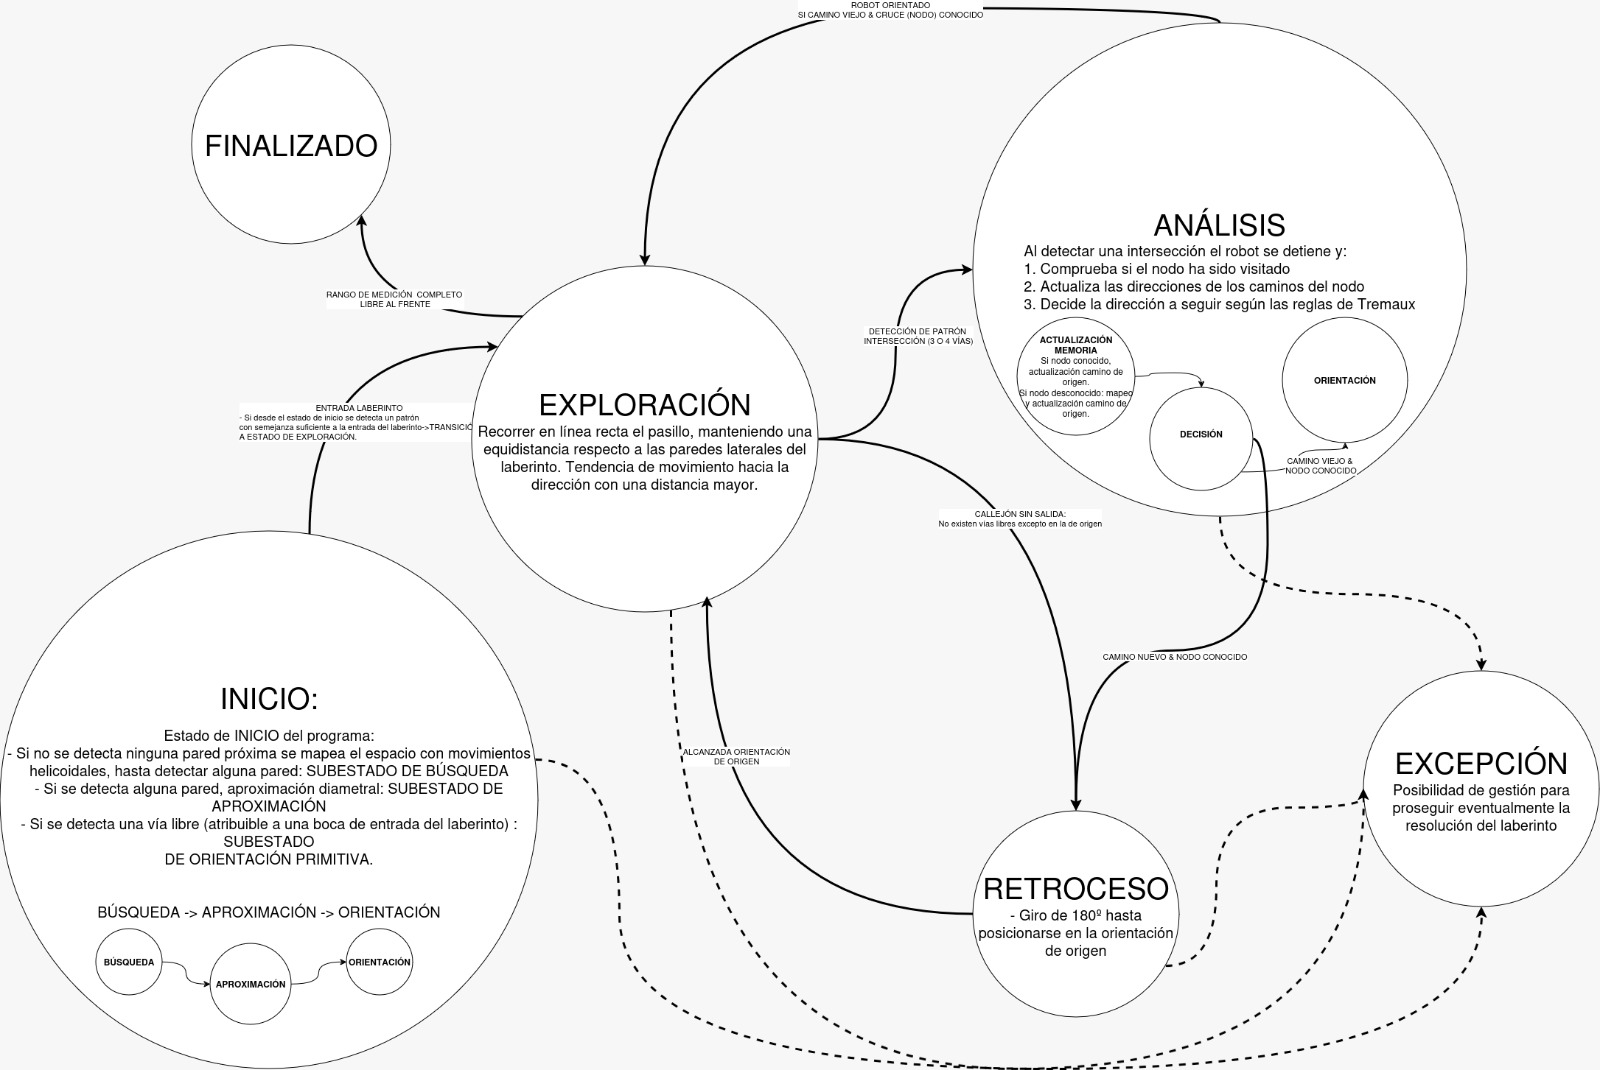
\includegraphics[width=0.9\textwidth]{Imágenes Memoria/Maquina_Tremaux.jpg}
    \caption{Máquina de estados de Trémaux}
    \label{fig:Tremaux}
\end{figure}


\subsubsection{Comportamiento Reactivo}
El último comportamiento que estudiamos se basa en una máquina de estados sencilla. Dos estados principales, \textit{E1} e \textit{Orientacion} se irán intercambiando dependiendo de la distancia a la que el robot se encuentre de la pared. Cuando el robot no se está orientando el \textit{E1} será el encargado de determinar lo que debe hacer el robot ya que es un \textit{superestado} que contendrá a suvez los estados: \textit{START}, \textit{AVANCE} y \textit{FIN}.
\paragraph{}
La idea de este algoritmo es orientar el robot de forma que siempre se dirija al espacio más abierto hasta que todas las distancias que detecte el láser sean próximas a infinito, momento en el que el robot se encontrará en el final del laberinto.

\begin{figure}[h!]
    \centering
    \begin{minipage}{0.45\textwidth}
        \centering
        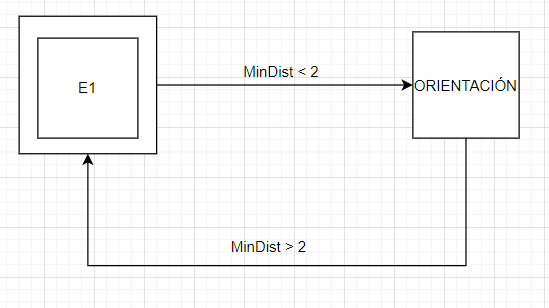
\includegraphics[width=\textwidth]{Imágenes Memoria/Diagrama_reactivo_1.PNG}
        \caption{Máquina de estados final del sigue paredes}
        \label{fig:Maquina de estados Reactiva}
    \end{minipage}%
    \hspace{0.05\textwidth} % Espacio entre las dos imágenes
    \begin{minipage}{0.45\textwidth}
        \centering
        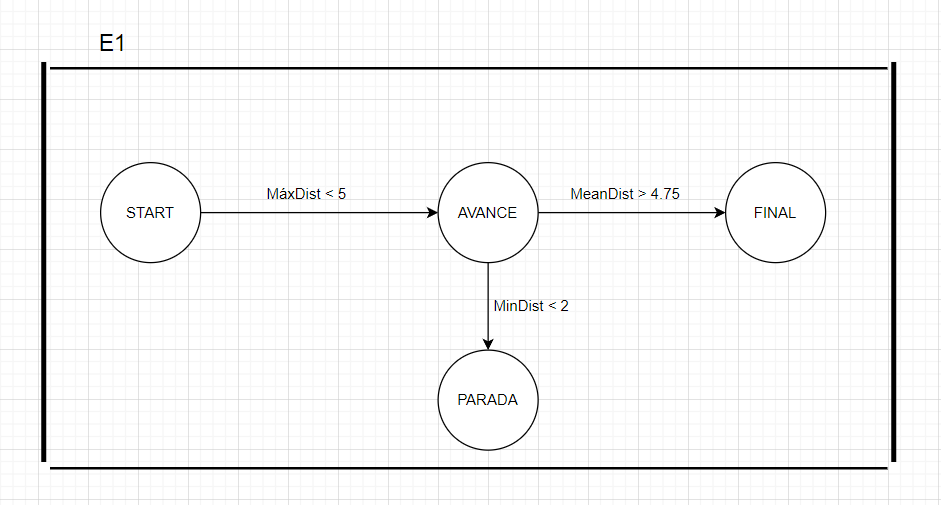
\includegraphics[width=\textwidth]{Imágenes Memoria/Diagrama_reactivo_2.PNG}
        \caption{Subestado}
        \label{fig:Subestado maquina reactiva}
    \end{minipage}
\end{figure}

Pese a lo sencillo del planteamiento esta máquina de estados ha resultado ser la más fácil de transportar a código 
pues sigue una lógica semejante a la que ya habíamos implementado en otras asignaturas para hacer prácticas con robots tales 
como el \textit{turtlebot}, que funciona de forma muy similar a nuestro robot simulado.

\subsection{Implementación del espacio de trabajo}
Lo primero que hicimos tras crear las máquinas de estados fue establecer un espacio de trabajo para ejecutar las pruebas pertinentes. Encontramos un \href{https://github.com/rfzeg/plywood_mazes}{repositorio}
que contenía varios mapas laberínticos, así que decidimos usar los modelos en nuestros paquetes para poder utilizarlos. Estos archivos .world usan plantillas que también tuvimos que añadir al paquete en 
una estructura anidada de archivo .sdf y .world.
\paragraph{}
Para cada uno de los mapas creamos su respectivo archivo \textit{.launch} y lo pusimos a funcionar. Por desgracia, el robot de ejemplo era demasiado grande para nuestro laberinto y apenas podía pasar entre 
las paredes así que diseñamos un nuevo modelo llamado \textit{robot pequeno} en el que redujimos a la mitad el tamaño de la caja, las ruedas y reubicamos los objetos de contacto frontal y trasero. Este cambio
implicó variar parámetros que ya estaban establecidos en nuestro programa de control, pues las aceleraciones y velocidades dependen de la masa de nuestro robot, que es calculada automáticamente por 
\href{https://gazebosim.org/home}{\textit{gazebo}}.
\paragraph{}
Por otro lado se han construido tres laberintos que ascienden en complejidad, aún que todos ellos cumplen el requisito de unicursalidad y ninguno presenta bucles.
El primero de ellos es simplemente un pasillo esquinado, por lo que el robot ha de llegar de un extremo a otro; el segundo de los laberintos le añade la dificultad de una bifurcación; 
y el tercero ya es un laberinto con mutitud de intersecciones y callejones sin salida.
\paragraph{}
La variedad de laberintos que utilizaremos nos permitirá recabar muchos datos, sobre todo gracias a la diversidad de forma y complejidad de los mismos. Aquí mostramos tan solo algunos de ellos:
\begin{figure}[h!]
    \centering
    \begin{minipage}{0.45\textwidth}
        \centering
        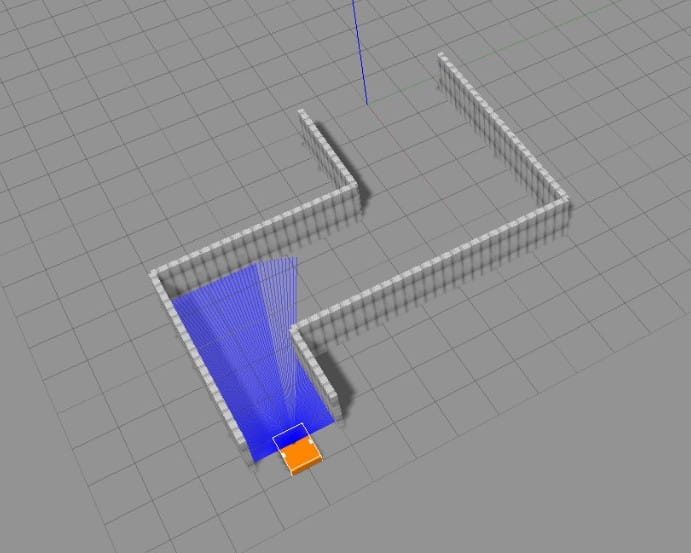
\includegraphics[width=\textwidth]{Imágenes Memoria/laberinto_01.jpeg}
        \caption{Laberinto 1}
        \label{fig:laberinto 1}
    \end{minipage}%
    \hspace{0.05\textwidth} % Espacio entre las dos imágenes
    \begin{minipage}{0.45\textwidth}
        \centering
        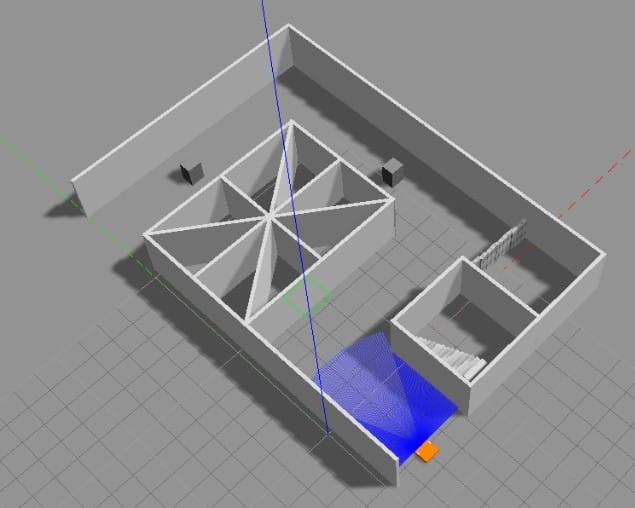
\includegraphics[width=\textwidth]{Imágenes Memoria/laberinto_02.jpeg}
        \caption{Laberinto 2}
        \label{fig:Laberinto 2}
    \end{minipage}
\end{figure}
\begin{figure}[h!]
    \centering
    \begin{minipage}{0.45\textwidth}
        \centering
        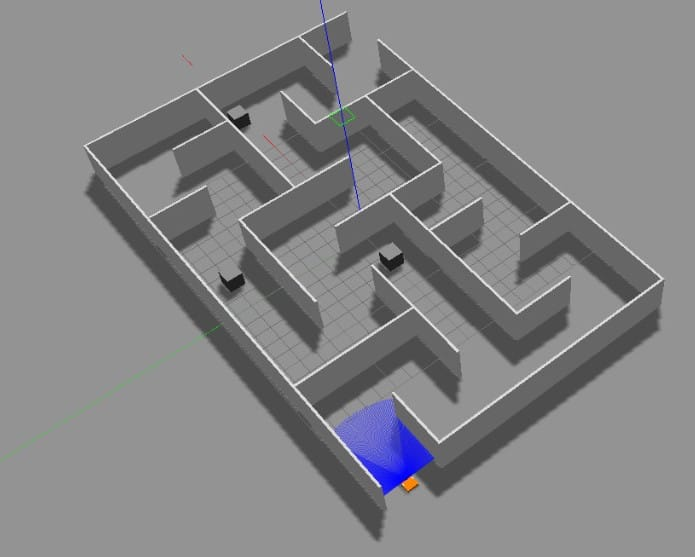
\includegraphics[width=\textwidth]{Imágenes Memoria/laberinto_03.jpeg}
        \caption{Laberinto 3}
        \label{fig:laberinto 3}
    \end{minipage}%
    \hspace{0.05\textwidth} % Espacio entre las dos imágenes
    \begin{minipage}{0.45\textwidth}
        \centering
        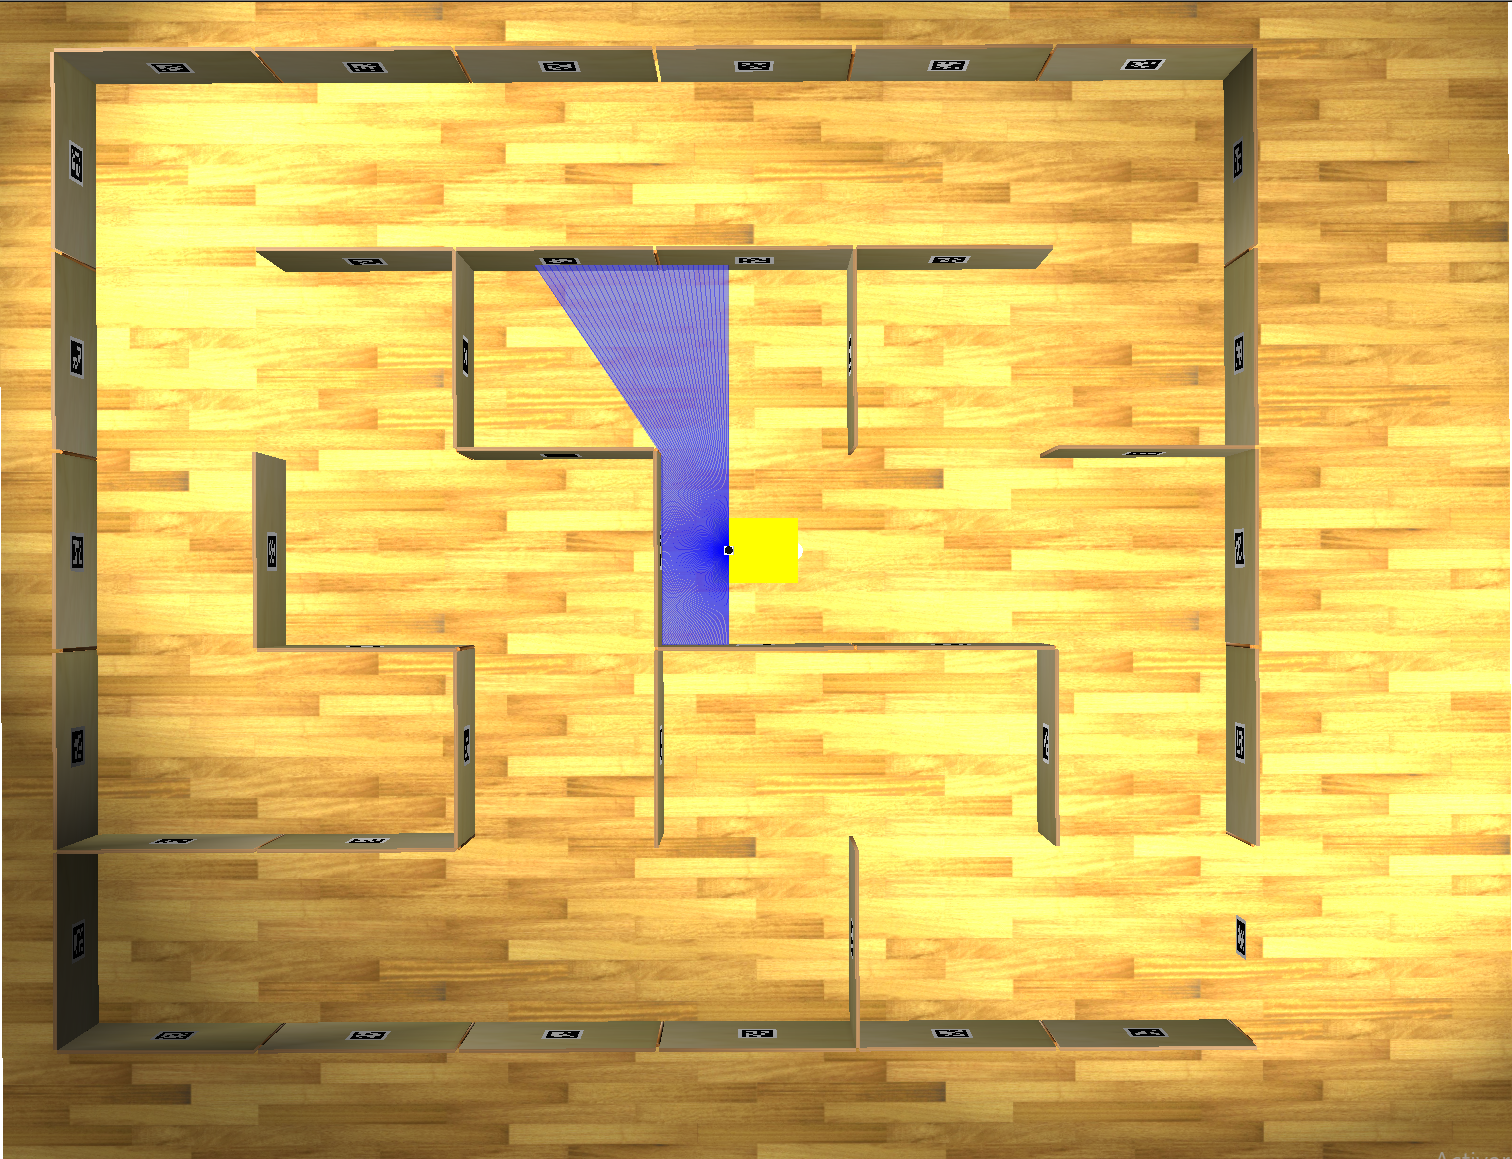
\includegraphics[width=\textwidth]{Imágenes Memoria/laberinto_04.PNG}
        \caption{Laberinto 4}
        \label{fig:Laberinto 4}
    \end{minipage}
\end{figure}


\subsection{Implementación del comportamiento}
El paso de máquina de estados a código Python resultó ser más complicado de lo esperado. La mejor forma de implementar un pseudocódigo como el de una máquina de estados sería 
creando una clase que contenga los objetos estado por los que pasará nuestro robot, pero no nos dimos cuenta hasta ya pasado tiempo desde que empezamos a diseñar los programas. 
\paragraph{}
No obstante, si que intentamos crear una clase que contuviese los estados para aplicar el seguidor de paredes al robot sin demasiado éxito pues la lógica de un seguidor de paredes
es algo que no se puede encapsular tan facilmente dentro de una clase, sobre todo, teniendo en cuenta la información tan poco depurada que nos proporciona el láser del robot.
\paragraph{}
También intentamos hacer lo mismo con el algoritmo de Trémaux, de igual forma, tuvimos poco éxito. Además de ser un algoritmo
bastante compljo por si solo, ser capaces de definir los estados con precisión solo teniendo en cuenta las distancias 
del robot y sin poder acceder a la odometría del mismo con precisión complican tremendamente programar un código que 
resuelva nuestros laberintos por simples que sean.
\paragraph{}
En ambos los casos anteriores si bien es cierto que el comportamiento no funciona en la puesta en práctica en el simulador 
creemos que sirven para ejemplificar como deberíamos pasar de una máquina finita de estados a una clase de Python. Pues 
la conversión si que es acertada.
\paragraph{}
El fracaso en los anteriores programas nos hizo plantearnos el algoritmo reactivo de forma ligeramente distinta, pues en 
vez de implementar una clase que transportase la MEF pensamos que nos sería más fácil aplicar una lógica de distnacias 
directamente sobre el robot aunque en cualquier caso, sí que dividimos los estados en funciones.
\paragraph{}
\textbf{Estados:}
\begin{itemize}
    \item \textbf{final}: Indica que el robot ha encontrado la salida. Si se activa, detiene el robot y finaliza el programa.
    \item \textbf{parar1}: Estado que indica que el robot ha detectado un obstáculo y debe detenerse, pero puede seguir orientándose.
    \item \textbf{parar}: Estado que indica que el robot debe parar completamente debido a obstáculos cercanos. En este estado, el robot ejecuta la función \texttt{orientar\_choque()} para evitar colisiones.
    \item \textbf{start}: El robot comienza su movimiento inicial. Se establece una velocidad hacia adelante.
    \item \textbf{adelante}: Indica que el robot avanza hacia adelante cuando no hay obstáculos cercanos.
    \item \textbf{retroceso}: Indica que el robot retrocede cuando detecta un obstáculo inminente.
\end{itemize}

\textbf{Condiciones y transiciones:}
\begin{itemize}
    \item \textbf{Detección de salida}: Si la media de los rangos de distancia es mayor que 4.75, se activa el estado \textbf{final}.
    \item \textbf{Detección de obstáculos}:
    \begin{itemize}
        \item Si el rango mínimo en la parte derecha es menor que 3.6, se activa el estado \textbf{adelante} como \textbf{False} y se activa \textbf{parar1}.
        \item Si hay un obstáculo cercano (menos de 2 metros) en cualquiera de los rangos (izquierda, derecha o media), se activa \textbf{parar}.
        \item Si el rango mínimo en cualquier dirección es cero, se activa el estado \textbf{retroceso}.
    \end{itemize}
    \item \textbf{Orientación y giro}: Dependiendo de las mediciones de distancia, se determina si el robot debe girar a la izquierda, a la derecha o continuar recto. Esto se maneja en las funciones \texttt{orientar()} y \texttt{orientar\_choque()}.
\end{itemize}
\textbf{Ciclo principal:}
\begin{itemize}
    \item Si \textbf{final} es \textbf{True}, se reporta el tiempo y la distancia total recorrida, y se detiene el robot.
    \item Si \textbf{parar1} o \textbf{parar} son \textbf{True}, el robot se detiene y se orienta según las condiciones de obstáculos.
    \item Si \textbf{start} o \textbf{adelante} son \textbf{True}, el robot avanza.
    \item Si \textbf{retroceso} es \textbf{True}, el robot retrocede.
    \item Si no se cumplen otras condiciones, se ejecuta \texttt{orientar\_choque()} para evitar colisiones.
\end{itemize}

\section{Conclusiones}
\subsection{Resultados del algoritmo reactivo}
Para probar el algoritmo reactivo se han utilizado todos los mapas del paquete excepto el \textit{maze 4 metal 6x6.world}.
En todos los casos, debido a la configuración de los laberintos, el robot ha sido capaz de llegar 
a la salida en tiempos muy semejantes, lo que nos hace pensar que el algoritmo reactivo es muy eficiente en laberintos unicursales. No obstante, debido a su comportamiento no afín a 
ningún algoritmo garantista, cabe la posibilidad de que en laberintos con otras configuraciones del espacio no demasiado diferentes el robot no sea capaz de llegar a la salida y pueda 
quedarse atascado en un bucle infinito o regresar al punto de partida. Respecto al requerimiento de esquivar obstaculos el robot ha sido capaz de hacerlo en todos los casos, aunque en 
alguno de los casos ha rozado con el, lo que se debe con alta probabilidad a la configuración de la respuesta del robot ante la distancia de los obstáculos. 
\paragraph{}
Por otra parte, en los laberintos del \href{https://github.com/rfzeg/plywood_mazes}{repositorio} nuestro robot no siempre alcanzó la 
meta pues al ser el espacio entre pasillos más pequeño la lógica de distancias lo hacía girar sobre sí mismo muchas veces.
Sin embargo, el editar las distancias clave de nuestro algoritmo sería suficiente para conseguir un comportamiento correcto.
\begin{table}[h!]
    \centering
    \begin{tabular}{|c|c|c|c|}
        \hline
        \textbf{Laberinto} & \textbf{Tiempo 1 (s)} & \textbf{Tiempo 2 (s)} & \textbf{Tiempo 3 (s)} \\
        \hline
        Laberinto 1 & 37.9 & 36.7 & 36.37 \\
        \hline
        Laberinto 2 & 75.21 & 77.91 & 74.50 \\
        \hline
        Laberinto 3 & 162.00 & 154.66 & 163.45 \\
        \hline
    \end{tabular}
    \caption{Tabla de resultados}
    \label{tabla:resultados}
\end{table}


%Video algoritmo 
Vídeos de demostración:
\begin{enumerate}
    \item\href{https://youtu.be/u6S0vK1PFoI}{Video laberinto empty}
    \item\href{https://www.youtube.com/watch?v=it0r5Ylg6to&ab_channel=Kit0s}{Video laberinto 01}
    \item\href{https://www.youtube.com/watch?v=SlumQXdpNc8&ab_channel=Kit0s}{Video laberinto 02}
\end{enumerate}
\subsection{Conclusiones finales}
En definitiva, podríamos decir que hemos implementado un código hijo de una máquina finita de estados para mover un 
robot de forma que sea capaz de salir por sí mismo de un laberinto. Pese a que este era el objetivo inicial el cual 
podríamos decir que hemos alcanzado no estamos del todo satisfechos con esta práctica.
\paragraph{}
Sabemos que dentro de la planificación de la materia esta práctica nos debería llevar un mes de curso aproximadamente, 
sin embargo, sentimos que con algo más de tiempo habríamos sido capaces de implementar comportamientos funcionales de verdad 
para laberintos mucho más complejos de los que hemos resuelto. Hay una infinidad de metodologías y algoritmos que nos 
hubiese gustado probar y desarrollar aplicando un nivel de profundidad más complejo a la resolución de laberintos. Herramientas 
tales como los algoritmos de búsqueda o las redes neuronales para la optimización del tiempo de resolución habrían sido interesantes
de estudiar.
\paragraph{}
De todos modos, sentimos que la parte de implementación de código ha quedado algo escasa pese a haber presentado un programa 
funcional. Ni Trémaux ni el seguidor de paredes se han conseguido implementar por lo que el programa final no se corresponde 
exactamente a una máquina de estados muy compleja y su código es incompleto dependiendo del laberinto al que nos enfrentemos.
\paragraph{}
En síntesis, hemos conseguido los objetivos de esta práctica, pero nos hubiese gustado dotado al robot de comportamientos 
más precisos para entornos más complejos.
% Bibliografía
\newpage
\begin{thebibliography}{8}

    \bibitem{Nuestro Repositorio }
    \href{https://github.com/MarcosFontenlos/Axentes_intelixentes}{Repositorio de \textit{MarcosFontenlos}}
    
    % Repositorio de los mapas
    \bibitem{mapas}
    \href{https://github.com/rfzeg/plywood_mazes}{Repositorio de \textit{rfzeg}}
    
    % Enlaces adicionales
    \bibitem{tremaux} Wikipedia, \textit{Algoritmo de Trémaux}. \url{https://es.wikipedia.org/wiki/Algoritmo_de_Tr%C3%A9maux} (Accedido: 2024).
    
    \bibitem{mdpi} Autor, \textit{Título del artículo}. MDPI, 2023. \url{https://www.mdpi.com/2227-7080/11/6/171} (Accedido: 2024).
    
    \bibitem{upcommons} Autor, \textit{Estudio e Implementación de un Algoritmo de Resolución de Laberintos utilizando Visión Artificial y un Robot Colaborativo}. UPC, 2023. \url{https://upcommons.upc.edu/bitstream/handle/2117/397735/Memoria%20TFE-%20ESTUDIO%20E%20IMPLEMENTACI%C3%93N%20DE%20UN%20ALGORITMO%20DE%20RESOLUCI%C3%93N%20DE%20LABERINTOS%2c%20UTILIZANDO%20VISI%C3%93N%20ARTIFICIAL%20Y%20UN%20ROBOT%20COLABORATIVO.pdf?sequence=2&isAllowed=y} (Accedido: 2024).
\end{thebibliography}

\end{document}